\documentclass[12pt,oneside]{book} % use larger type; default would be 10pt

\usepackage[utf8]{inputenc} 
\usepackage[czech]{babel}
\usepackage[IL2]{fontenc}
\usepackage[a4paper]{geometry} 
\usepackage[pdftex]{graphicx} 
\usepackage[parfill]{parskip} 		% Activate to begin paragraphs with an empty line rather than an indent
\usepackage[explicit]{titlesec}
\usepackage{titletoc}
\usepackage{multirow}
\usepackage{bytefield}
\usepackage{rotating}
\usepackage{booktabs}  			% for much better looking tables
\usepackage{longtable}
\usepackage{lscape}
\usepackage{array} 	  		% for better arrays (eg matrices) in maths
\usepackage{paralist}  			% very flexible & customisable lists (eg. enumerate/itemize, etc.)
\usepackage{verbatim}  			% adds environment for commenting out blocks of text & for better verbatim
\usepackage{subfig}    			% make it possible to include more than one captioned figure/table in a single float
\usepackage[nottoc,notlof,notlot]{tocbibind} % Put the bibliography in the ToC
\usepackage[titles,subfigure]{tocloft}		 % Alter the style of the Table of Contents
\usepackage{color}
\usepackage[usenames,dvipsnames]{xcolor}
\usepackage{pdfmarginpar}
\usepackage{lastpage}
\usepackage{circuitikz}
\usepackage{tikz}
\usetikzlibrary{shapes,arrows,positioning,snakes,backgrounds,decorations.footprints,shadows,calc,chains} 
\usepackage{wrapfig}
\usepackage{listings}
\usepackage{tabularx}
\usepackage{enumitem}
\usepackage{anyfontsize}
\usepackage[pdftex, colorlinks=true, linkcolor=blue, urlcolor=blue]{hyperref} %should be last

\geometry{papersize={210mm,305mm},total={176mm,260mm}}

\usepackage{fancyhdr} % This should be set AFTER setting up the page geometry

\usepackage[local]{gitinfo2}

\pagestyle{fancyplain}     % options: empty , plain , fancy

\def\projectname{B5: Piano Tales Master}
\def\projectsubname{BROB - Základy robotiky\\[0.5cm]2019}
\def\projectdoc{Dokumentace projektu}

\definecolor{darkgray}{rgb}{0.4,0.4,0.9}
\definecolor{lightdarkgray}{rgb}{0.6,0.6,1.0}

\newcommand{\HRule}{\textcolor{darkgray}{\rule{\linewidth}{2mm}}}

\renewcommand{\headrulewidth}{1mm}
\renewcommand{\footrulewidth}{1mm}
\renewcommand{\plainheadrulewidth}{1mm}
\renewcommand{\plainfootrulewidth}{1mm}

\newcommand{\headrulecolor}{darkgray}
\newcommand{\footrulecolor}{darkgray}

\let\oldheadrule\headrule
\let\oldfootrule\footrule
\def\headrule{\textcolor{\headrulecolor}{\oldheadrule}}
\def\footrule{\textcolor{\footrulecolor}{\oldfootrule}}


\lhead{\projectdoc}
\chead{}
\rhead{\LARGE \projectname}
\lfoot{}
\cfoot{}
\rfoot{\thepage/\pageref{LastPage}}

\voffset 5mm
\setlength\headsep{8mm}

\newcommand{\up}[1]{\begin{sideways}\parbox{15mm}{#1}\end{sideways}}
\newcommand{\bx}[1]{\parbox{0.4\textwidth}{\centering #1}}

\tikzstyle{isipka} = [very thick,fill=none,rounded corners=2mm, color=red!100]
\tikzstyle{iodkaz} = [very thick,fill=none,rounded corners=3mm, color=red!100,line cap=round,align=center]
\tikzstyle{iprvek} = [rectangle, draw=red, rounded corners=3mm, line width=1mm]

\tikzstyle{postup} = [rectangle, draw, rounded corners=3mm, line width=1mm,minimum width=4cm,font=\bf]
\tikzstyle{labl} = [circle, draw, fill=white, rounded corners=3mm, line width=1mm,anchor=east,font=\bf]
\tikzstyle{edg} = [->, line width=1mm]

\tikzstyle{key} = [draw, fill=white, rectangle, rounded corners=2pt, inner sep=4pt, line width=0.5pt, drop shadow={shadow xshift=0.25ex,shadow yshift=-0.25ex,fill=black,opacity=0.75}, font=\scriptsize\sffamily, minimum height=1.5\baselineskip, minimum width=1.5\baselineskip]
\setcounter{secnumdepth}{-1}
\setcounter{tocdepth}{1}

\renewcommand\thepart{\arabic{part}}

\titleformat{\part}
  {\normalfont\normalsize}
  {}
  {20pt}
  {\begin{tikzpicture}[remember picture,overlay]%
	 \fill[lightdarkgray]  (current page.north west) rectangle ([yshift=-13cm]current page.north east);   
	 \node[fill=darkgray, text width=2\paperwidth, rounded corners=6cm, text depth=18cm, anchor=center, inner sep=0pt] at (current page.north east) (parttop) {\strut};
	 \node[anchor=south east, inner sep=0pt,	outer sep=0pt] at ([shift={(-2cm, +1cm)}]parttop.south)  (partnum) {\fontsize{10cm}{10}\selectfont\color{black}\thepart};
	 \node[anchor=north, inner sep=0pt]  at ([yshift=-2pt]partnum.south) (partname) {\large\scshape\bfseries\color{white} ČÁST};
 	 \node[anchor=north east, align=right, inner sep=0pt, outer ysep=2cm] at ([xshift=1cm]partnum.south) {\parbox{.7\textwidth}{\Huge\bfseries\raggedleft\projectname\\#1}};
 	 \node[anchor=north, align=left] at ([yshift=-12.5cm]current page.north) {\parbox{\textwidth}{\startcontents[part]\printcontents[part]{l}{0}{\setcounter{tocdepth}{0}}}};
   \end{tikzpicture}%    
  }

\titleformat{\chapter}
  {\normalfont}%
  {}%
  {20pt}%
  {\begin{tikzpicture}[remember picture,overlay]
    \fill[darkgray] (current page.north west) rectangle ([yshift=-3.5cm]current page.north east);
    \node[anchor=west, align=left, inner xsep=2cm] at ([yshift=-2cm]current page.north west) {\parbox{\textwidth}{\huge\sffamily\bfseries\scshape\color{white}#1}};%
   \end{tikzpicture}%
  }

\titlespacing*{\chapter}{0pt}{50pt}{-70pt}




\begin{document}
	
\begin{titlepage}
    \begin{center}

	~\\[0.5cm]
       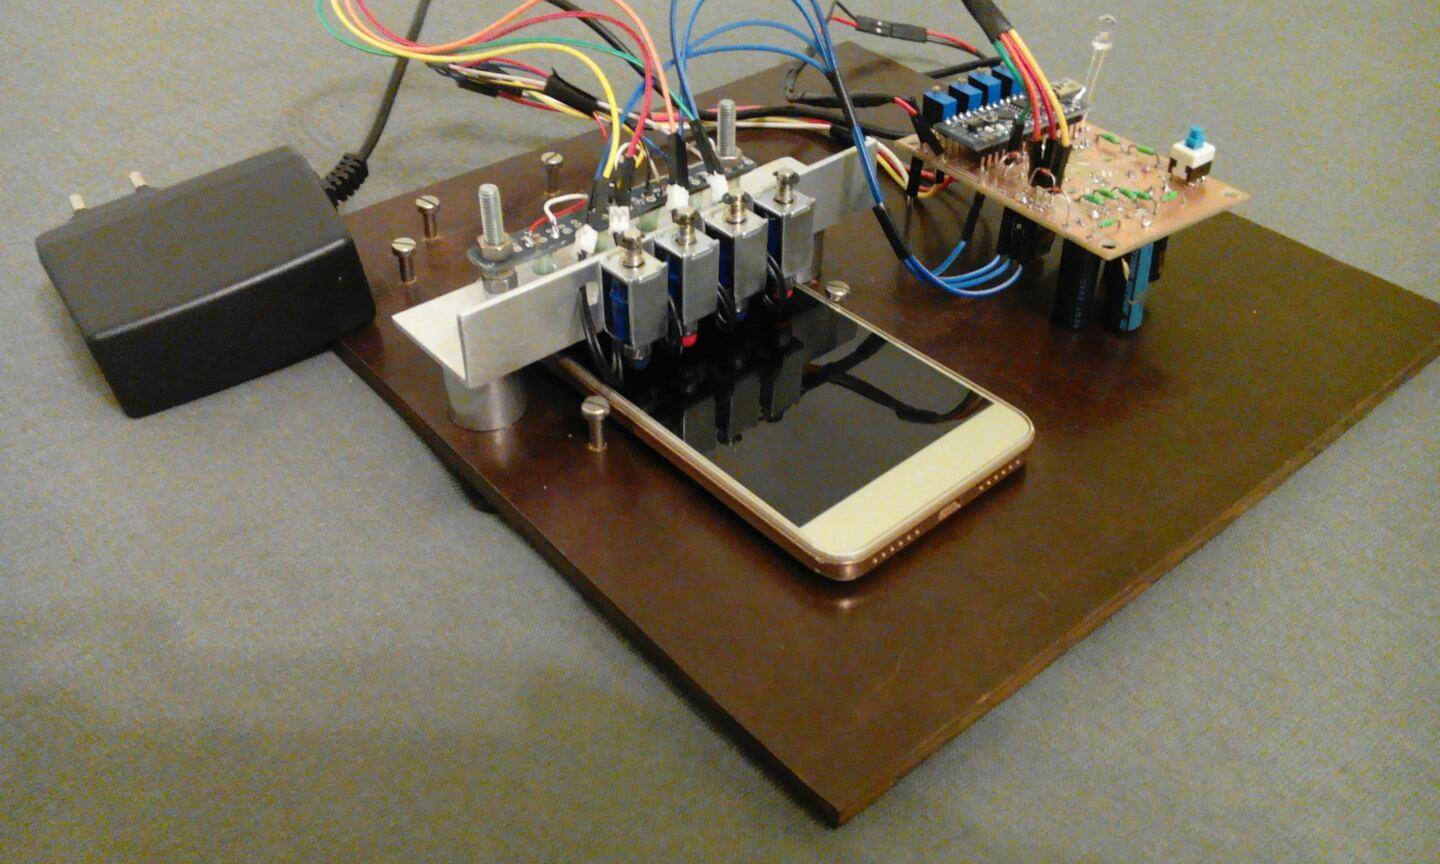
\includegraphics[width=0.85\textwidth]{./img/uvodka.jpg}\\[0cm] 

	~\\[2cm]

    % Title
    \HRule \\[0.4cm]
    { \huge \bfseries \projectname}\\[0.4cm]
       \textsc{\LARGE \projectsubname}\\[0.4cm]
    \HRule \\[1cm]
    
    \textsc{\LARGE \projectdoc}\\[0.5cm]
    \texttt{\Large \gitFirstTagDescribe}\\[1.5cm]

    % Author and supervisor
    \begin{minipage}{0.5\textwidth}
      \begin{center} \large
        
\includegraphics[width=0.85\textwidth]{./img/loga/vut.png}\\[1cm] 
		 \Large\bfseries UAMT FEKT VUT		
      \end{center}
    \end{minipage}%
    \begin{minipage}{0.5\textwidth}\raggedleft\Large\bfseries
 	Lukáš Zezula\par
        Dominik Řičánek\par
    \raggedright    
        Vedoucí projektu: \par
   \raggedleft     
        ing.Adam Ligocki
    \end{minipage}
    \vfill
   \end{center}
\end{titlepage}

\tableofcontents

%%%%%%%%%%%%%%%%%%%%%%%%%%%%%%%%%%%%%%%%%%%%%%%%%%%%%%%%%%%%%%%%%%%%%%%%%%%%%%%%%
%%%%%%%%%%%%%%%%%%%%%%%%%%%%%%%%%%%%%%%%%%%%%%%%%%%%%%%%%%%%%%%%%%%%%%%%%%%%%%%%%
%%%%%%%%%%%%%%%%%%%%%%%%%%%%%%%%%%%%%%%%%%%%%%%%%%%%%%%%%%%%%%%%%%%%%%%%%%%%%%%%%
%%%%%%%%%%%%%%%%%%%%%%%%%%%%%%%%%%%%%%%%%%%%%%%%%%%%%%%%%%%%%%%%%%%%%%%%%%%%%%%%%
\chapter{Analýza zadání}\label{analyza-zadani}
\section{Zadání}
\qquad Vytvořte robota, který bude hrát Piano Tales. Navrhněte stroj, který pomocí Vámi zvoleného HW (snímače a výpočetní jednotky a motorků) bude schopen hrát a porazit člověka ve hře Piano Tales. Referenčním výsledkem bude https://www.youtube.com/watch?v=fqOW84ZTL7k který se pokusíme porazit. Na závěr vznikne krátké propagační video na youtube obsahujcí logo VUT.
Projekt bude veden pomoci GITu. Dokumentace bude vytvořená v LaTeXu. 
\section{Úvod}\label{uvod}
\qquad Cílem projektu, jak je patrno ze zadání, bylo realizovat robota, který by hrál hru Piano Tales a dosahoval lepších výsledků než člověk a ideálně se přiblížil, nebo dokonce překonal referenční výsledek.

\qquad Hra Piano Tales funguje tak, že po obrazovce ve čtyřech lajnách jezdí obdélníky, jejichž stisknutím se zvýší skóre a rychlost s jakou se pohybují. Hra se tedy neustále ztěžuje. Jakmile nezachytíte již zmiňovaný obdélník nebo kliknete mimo jeho plochu, hra končí. Krom těchto obdélníků, které mají pevně definované rozměry, jezdí po obrazovce i delší obdélníkové úseky, které mají stálou šířku, ale jejich délka se různí (viz. Obrázek \ref{pianotales}). Tyto úseky se liší i barevně. Zatímco obdélníky jsou vždy striktně černé, tak barva úseků se mění od černé na začátku úseku po světlejší odstíny modré na konci. Přidržením těchto úseků od počátku do konce se skóre zvýší více než při pouhém stisknutí. 

\begin{figure}[h] \large\centering
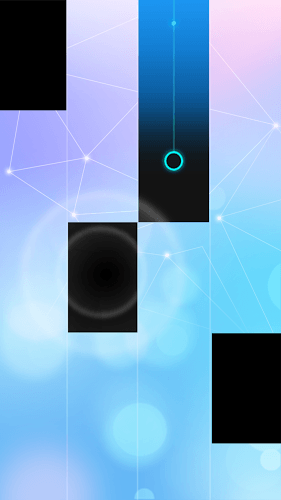
\includegraphics[width=0.30\textwidth]{./img/pianotales.png}\\[1cm] 
\caption{Ukázka hrací plochy hry Piano Tales}
\label{pianotales}
\end{figure}   
      
\section{Nástin řešení}\label{nastin}
\qquad Oproti videu, přiloženému k zadání, jsme neměli k dispozici tablet, kolem kterého by se dali pohodlně rozmístit servomotory, a proto jsme museli použít smartphone, který má podstatně menší rozměry. Toto vedlo na nutnost pracovat s menšími prvky, které by ovládaly dotykový display a složitější mechanickou konstrukci.

\qquad Nejvhodnější se ukázalo být použití elektromagnetů, konkrétně push type solenoidů, které byly pomocí mechanické konstrukce umístěny nad smartphonem tak, aby po přivedení napětí na řídící obvod stiskly specifické místo na dotykovém displayi.

\qquad Ke snímání průběhů obdélníků byly použiti fotorezistory. Tyto byly umístěny dostatečně blízko displaye a ve speciálně vytvořeném pouzdru, aby se minimalizoval vliv okolního osvětlení. 

\qquad Zjednodušený princip, s jakým výsledný robot hraje hru lze vidět na Obrázku \ref{blok_0}. Obdélník, mající černou barvu, se pohybuje po světle modrém pozadí kolem fotorezistoru. To zapříčiní změnu odporu, kterou zachycuje mikroprocesor a měří čas mezi přechody modrá-černá, černá-modrá. Z tohoto času a známých rozměrů obdélníku se vypočte rychlost, s kterou se obdélník pohybuje. Po započítání dopravního zpoždění, které je dáno zejména časem potřebným k sepnutí solenoidu, se určí okamžik, kdy přesně má být přiveden z mikroprocesoru spínací signál na vstup řídícího obvodu.

\begin{figure}[h] \large\centering
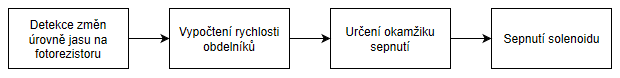
\includegraphics[width=0.80\textwidth]{./img/blok_0.png}\\[1cm] 
\caption{Zjednodušený princip funkce robotu}
\label{blok_0}
\end{figure}   
%%%%%%%%%%%%%%%%%%%%%%%%%%%%%%%%%%%%%%%%%%%%%%%%%%%%%%%%%%%%%%%%%%%%%%%%%%%%%%%%%
%%%%%%%%%%%%%%%%%%%%%%%%%%%%%%%%%%%%%%%%%%%%%%%%%%%%%%%%%%%%%%%%%%%%%%%%%%%%%%%%%
%%%%%%%%%%%%%%%%%%%%%%%%%%%%%%%%%%%%%%%%%%%%%%%%%%%%%%%%%%%%%%%%%%%%%%%%%%%%%%%%%
%%%%%%%%%%%%%%%%%%%%%%%%%%%%%%%%%%%%%%%%%%%%%%%%%%%%%%%%%%%%%%%%%%%%%%%%%%%%%%%%%
\part{MECHANICKÁ ČÁST}\label{mechanika}
\chapter{Návrh v prostředí AutoCAD}\label{CAD}

\begin{figure}[h]\large\centering
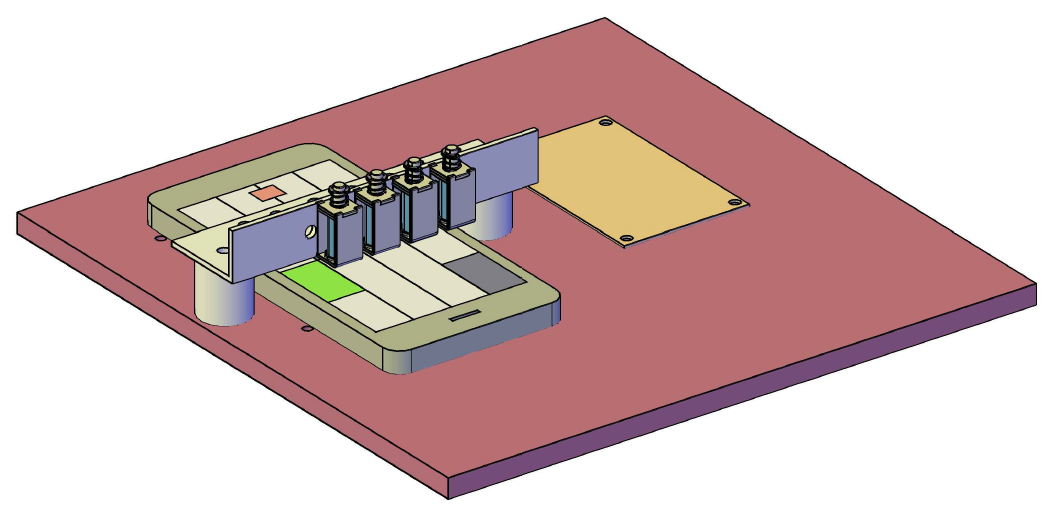
\includegraphics[width=1.00\textwidth]{./img/mech_cad0.png}\\[1cm] 
\caption{Model mechanické části v prostředí AutoCAD jiho-západní pohled}
\label{mech_cad0}
\end{figure}  

\begin{figure}[h]\large\centering
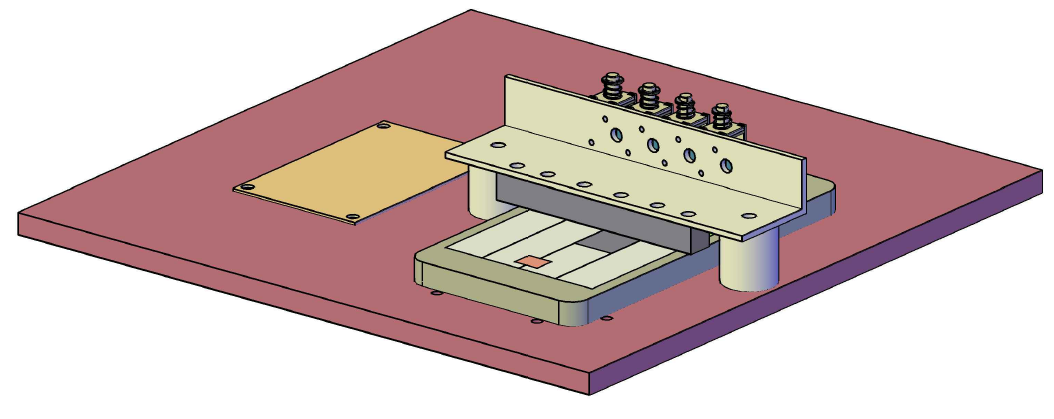
\includegraphics[width=1.00\textwidth]{./img/mech_cad1.png}\\[1cm] 
\caption{Model mechanické části v prostředí AutoCAD severo-západní pohled}
\label{mech_cad1}
\end{figure}  

\pagebreak

\section{Popis částí modelu}\label{mech_casti}
\qquad Model byl pomyslně rozdělen na 5 částí. Konkrétně se jedná o podstavu, L-profil, válcové spojky, solenoidy a pouzdro na fotorezistory. Tyto části jsou navrženy tak, aby byly demontovatelné (spoje jsou realizovány pouze šrouby a případně maticemi). Jak na sebe jednotlivé části navazují můžeme vidět na Obrázku \ref{mech_cad0} a \ref{mech_cad1}. Oranžový obdélníkový profil představuje plošný spoj.

\textbf{podstava}

\qquad Uchycením všech částí konstrukce pevně na podstavu čtvercového tvaru jsme předešli nežádoucím posuvům a docílili větší stability konstrukce. Více o nákresu a rozměrech podstavy viz. Příloha \hyperref[Prilohy]{1}.

\textbf{L-profil}

\qquad Tento ukotvuje solenoidy a pouzdro na fotorezistory. Je připevněn na válcové spojky, aby byl ve správné výšce nad smartphonem. Náčrt L-profilu lze vidět na Obrázku \ref{lprof}. Více o nákresu a rozměrech L-profilu viz. Příloha \hyperref[Prilohy]{1}.  

\begin{figure}[h] \large\centering
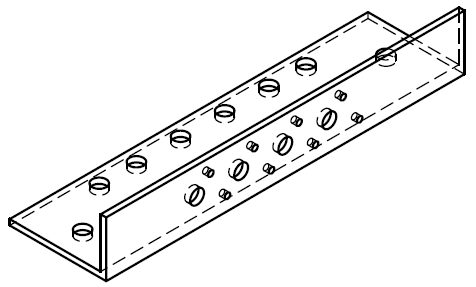
\includegraphics[width=0.60\textwidth]{./img/lprof.png}\\[1cm] 
\caption{Náčrt L-profilu}
\label{lprof}
\end{figure}   

\textbf{válcové spojky}

\qquad Jejich hlavní funkce spočívá v přichycení L-profilu k podstavě ve správné výšce tak, aby při sepnutí solenoidu došlo k interakci stylusu, umístěném na solenoidu, s dotykovým displayem. Rozměry válcových spojek byly tedy voleny tak, aby při zahrnutí tloušťky smartphonu (cca 9mm), výšky stylusu (cca 9,5mm) a zdvihu solenoidu (cca 3.5mm) došlo po přivedení napětí k již zmíněnému dotyku.  Více o nákresu a rozměrech válcových spojek viz. Příloha \hyperref[Prilohy]{1}.


\textbf{solenoidy}

\qquad Jak již bylo zmíněno v \hyperref[nastin]{Nástinu řešení} museli být použity součástky, které by se dali umístit kolem poměrně malého smartphonu. Pro tento účel jsme vybrali push type solenoidy se zdvihem okolo 3.5mm a rozměry takovými, aby se na šířku smartphonu (cca 74mm) vlezli alespoň 4 tyto solenoidy. Konkrétní rozměry solenoidů lze vyčíst z datasheetu viz. Příloha \hyperref[Prilohy]{4}. 3D model solenoidu byl převzat ze stránek GRABCAD COMMUNITY. \cite{grabcad}

\pagebreak
\textbf{pouzdro na fotorezistory}

\qquad Jeho hlavní význam spočívá v odstínění okolního osvětlení a ukotvení fotorezistorů na požadované místo. Je přichycen k L-profilu a umístěn v takové výšce nad smartphonem, aby fotorezistory dostatečně dobře snímali změny jasu na displayi a zároveň nebyly příliš ovlivněny osvětlením místnosti. Fotorezistory jsou v pouzdru zapuštěny cca 1mm a jsou vzdáleny od smartphonu cca 4mm. Náčrt pouzdra lze vidět na Obrázku \ref{pouzdro}. Více o nákresu a rozměrech pouzdra na fotorezistory viz. Příloha \hyperref[Prilohy]{1}.

\begin{figure}[h] \large\centering
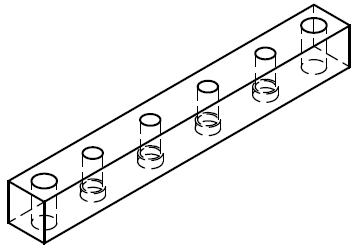
\includegraphics[width=0.60\textwidth]{./img/pouzdro.png}\\[1cm] 
\caption{Náčrt pouzdra na fotorezistory}
\label{pouzdro}
\end{figure}  

\chapter{Konstrukce mechanické části}\label{konstr}
\qquad Všechny části konstrukce byly nařezány, obroušeny a byly do nich navrtány díry a závity dle výkresové dokumentace (viz. Příloha \hyperref[Prilohy]{1}).

\qquad Jako materiál pro podstavu byl zvolen akryl, hlavně díky jeho dostupnosti a kvalitním izolačním vlastnostem. Závity, které se nacházejí kolem smartphonu a lze je vidět na Obrázku \ref{mech_cad0} a \ref{mech_cad1}, slouží pro šrouby M4, které nebyly zašroubovány na doraz proto, aby se mezi ně dal zasunout smartphone a tím byl pevně uchycen na jedno místo. K podstavě byla přišroubována deska plošných spojů.

\qquad Válcové spojky a L-profil byly odříznuty z hliníkových profilů (konkrétně typ AlMgSi0,5). K válcovým spojkám je z jedné strany šroubem M5 přišroubovaná podstava a z druhé L-profil. K L-profilu je poté pomocí šroubů M5 a matic přichyceno pouzdro na fotorezistory a tyto jsou připájeny na kousek univerzálního pájivého pole, odkud potom vedou dráty na plošný spoj. 

\qquad Do rámu solenoidů byly do předchystaných děr vyřezány závity M2 a následně jsme solenoidy přišroubovaly k L-profilu.Napájecí kabely solenoidů jsme protáhly příslušnými dírami a přivedli na desku plošných spojů. Stylusy byly, vzhledem k jejich malým rozměrům a faktu, že by nevydržely obráběni, k solenoidům přilepeny tekutým kovem (WURTH tekutý kov FE1).

\qquad Na závěr bylo nutné zajistit, aby se přívodní drátky fotorezistorů nemohli dotknout hliníkového L-profilu. Toho bylo dosaženo umístěním odstřižků plastových slámek kolem zmíněný drátků. 

\qquad Vybrané snímky z konstrukce mechanické části lze vidět na Obrázku \ref{konstr0} a \ref{konstr1}

\begin{figure}[h] \large\centering
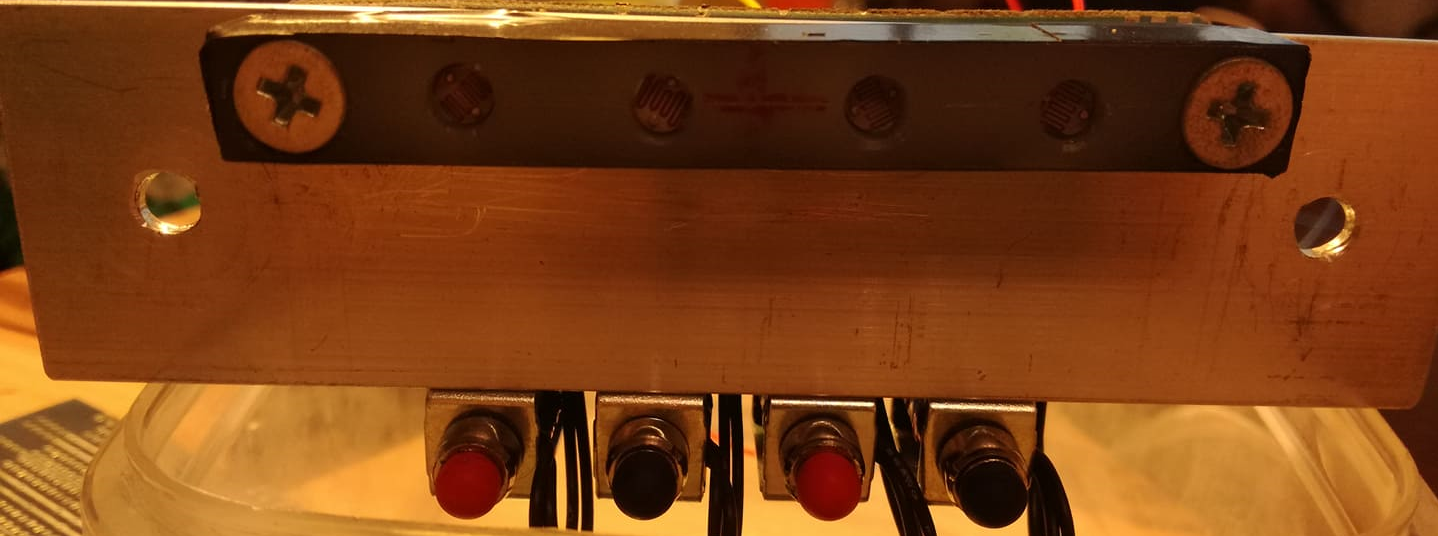
\includegraphics[width=0.80\textwidth]{./img/konstr0.png}\\[1cm] 
\caption{Fotka spodní části L-profilu s přichycenými solenoidy a pouzdrem na fotorezistory}
\label{konstr0}
\end{figure} 

\begin{figure}[h] \large\centering
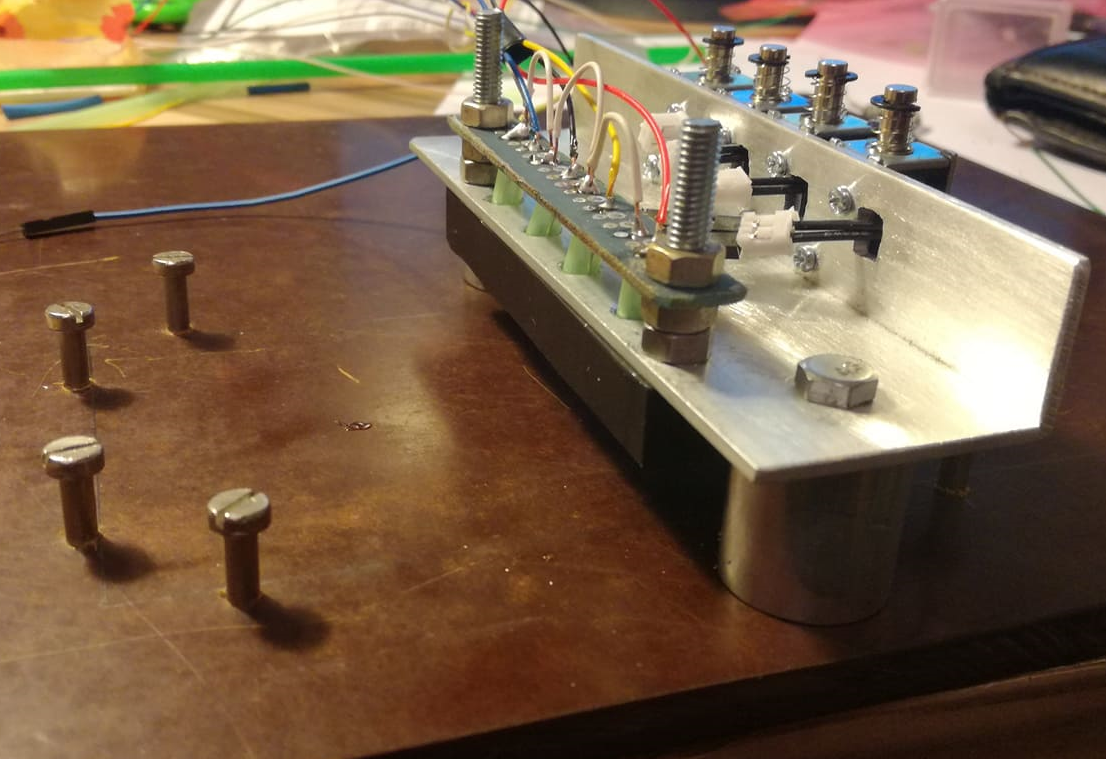
\includegraphics[width=1.00\textwidth]{./img/konstr1.png}\\[1cm] 
\caption{Fotka mechanické konstrukce - severo-západní pohled}
\label{konstr1}
\end{figure} 
%%%%%%%%%%%%%%%%%%%%%%%%%%%%%%%%%%%%%%%%%%%%%%%%%%%%%%%%%%%%%%%%%%%%%%%%%%%%%%%%%
%%%%%%%%%%%%%%%%%%%%%%%%%%%%%%%%%%%%%%%%%%%%%%%%%%%%%%%%%%%%%%%%%%%%%%%%%%%%%%%%%
%%%%%%%%%%%%%%%%%%%%%%%%%%%%%%%%%%%%%%%%%%%%%%%%%%%%%%%%%%%%%%%%%%%%%%%%%%%%%%%%%
%%%%%%%%%%%%%%%%%%%%%%%%%%%%%%%%%%%%%%%%%%%%%%%%%%%%%%%%%%%%%%%%%%%%%%%%%%%%%%%%%
\part{Návrh a realizace elektronické části}\label{elektro}

\chapter{BLABLA}\label{BLABLA}
\section{2xBLABLA}\label{2xBLABLA}

%%%%%%%%%%%%%%%%%%%%%%%%%%%%%%%%%%%%%%%%%%%%%%%%%%%%%%%%%%%%%%%%%%%%%%%%%%%%%%%%%
%%%%%%%%%%%%%%%%%%%%%%%%%%%%%%%%%%%%%%%%%%%%%%%%%%%%%%%%%%%%%%%%%%%%%%%%%%%%%%%%%
%%%%%%%%%%%%%%%%%%%%%%%%%%%%%%%%%%%%%%%%%%%%%%%%%%%%%%%%%%%%%%%%%%%%%%%%%%%%%%%%%
%%%%%%%%%%%%%%%%%%%%%%%%%%%%%%%%%%%%%%%%%%%%%%%%%%%%%%%%%%%%%%%%%%%%%%%%%%%%%%%%%
\part{Programová část}\label{program}

\chapter{Úvod}\label{progUvod}
\section{Řešení}\label{progRes}
\qquad Problém, který jsme museli vyřešit byl, jak co nejrychleji zajistit snímání hrací plochy a samotné hraní za použití mechanických prstů. Zde jsme měli na výběr z vícero možností. \par  1. Použít kameru s rychlostí snímání alespoň stejnou, nebo větší než je rychlost FPS na hracím mobilu a vyhodnocovat každý snímek digitálně za pomoci počítačového vidění \\ 2. Použít analogové senzory a vyhodnocovat úrovně signálu.\par \qquad Jelikož jsme se domnívali, že takovový software na zpracovávání obrazu bychom si museli sami vytvořit (což podle by mohl být projekt sám o sobě) zvolili jsme cestu analogových senzorů, které zpracováváme přes čtyři AD převodníky v kopii arduino nano. Dalo by se spekulovat která z možností by byla vhodnější, obě mají své pro a proti a obě by ve výsledku vyšli stejně časově náročné.

\section{Volba jazyka}
\qquad Jak už bylo řečeno, náš projekt běží na identické kopii arduino nano (konkrétně je to Nano3, ale na tom nezáleží), takže jsme mohli programovat v C nebo C++ přičemž na náš projekt se velmi hodilo objektové programování, a taky jsem si to chtěl vyzkoušet, takže ve výsledku je header.h napsán v C++ a celý robot je ovládán metodamy v hlavní smyčce.

\chapter{Návod}\label{progNavod}
\section{Návod k použití}
\qquad Před započetím hry je nutné PianoTilesMaster zkalibrovat. A to z důvodu použitých LDR jako senzorů, ty se můžou vychýlovat podle změn okolního jasu. \par Kalibrace se provádí ihned po zapnutí nebo restartu mikrokontroleru a pro novou kalibraci se musí znovu restartovat. Hned po zapnutí se rosvítí kontrolní LED na pinu 11 a program čeká na stisknutí tlačítka na pinu 12. Jako referenční senzor ke kalibraci se používá první senzor z prava. \par \qquad První pod referenční senzor dáme černý čtvereček a zmáčkneme tlačítko. LED se na chvíli zhasne a posléze znovu rosvítí. Posuneme pod ref. senzor pozadí hrací plochy a znovu zmáčkneme tlačítko. Tentokrát LED zabliká, to signalizuje, že je program připraven k chodu a mělo by všechno věžet v pořádku, po následovném stisku tlačítka LED zhasne a PianoTilesMaster počítá s tím, že hra už běží. \par \qquad Kdykoliv za chodu programu je možné PianoTilesMaster pozastavit stiskem tlačítka a opětovným stiskem jej znovu spustit.

\begin{figure}[h]\small\centering
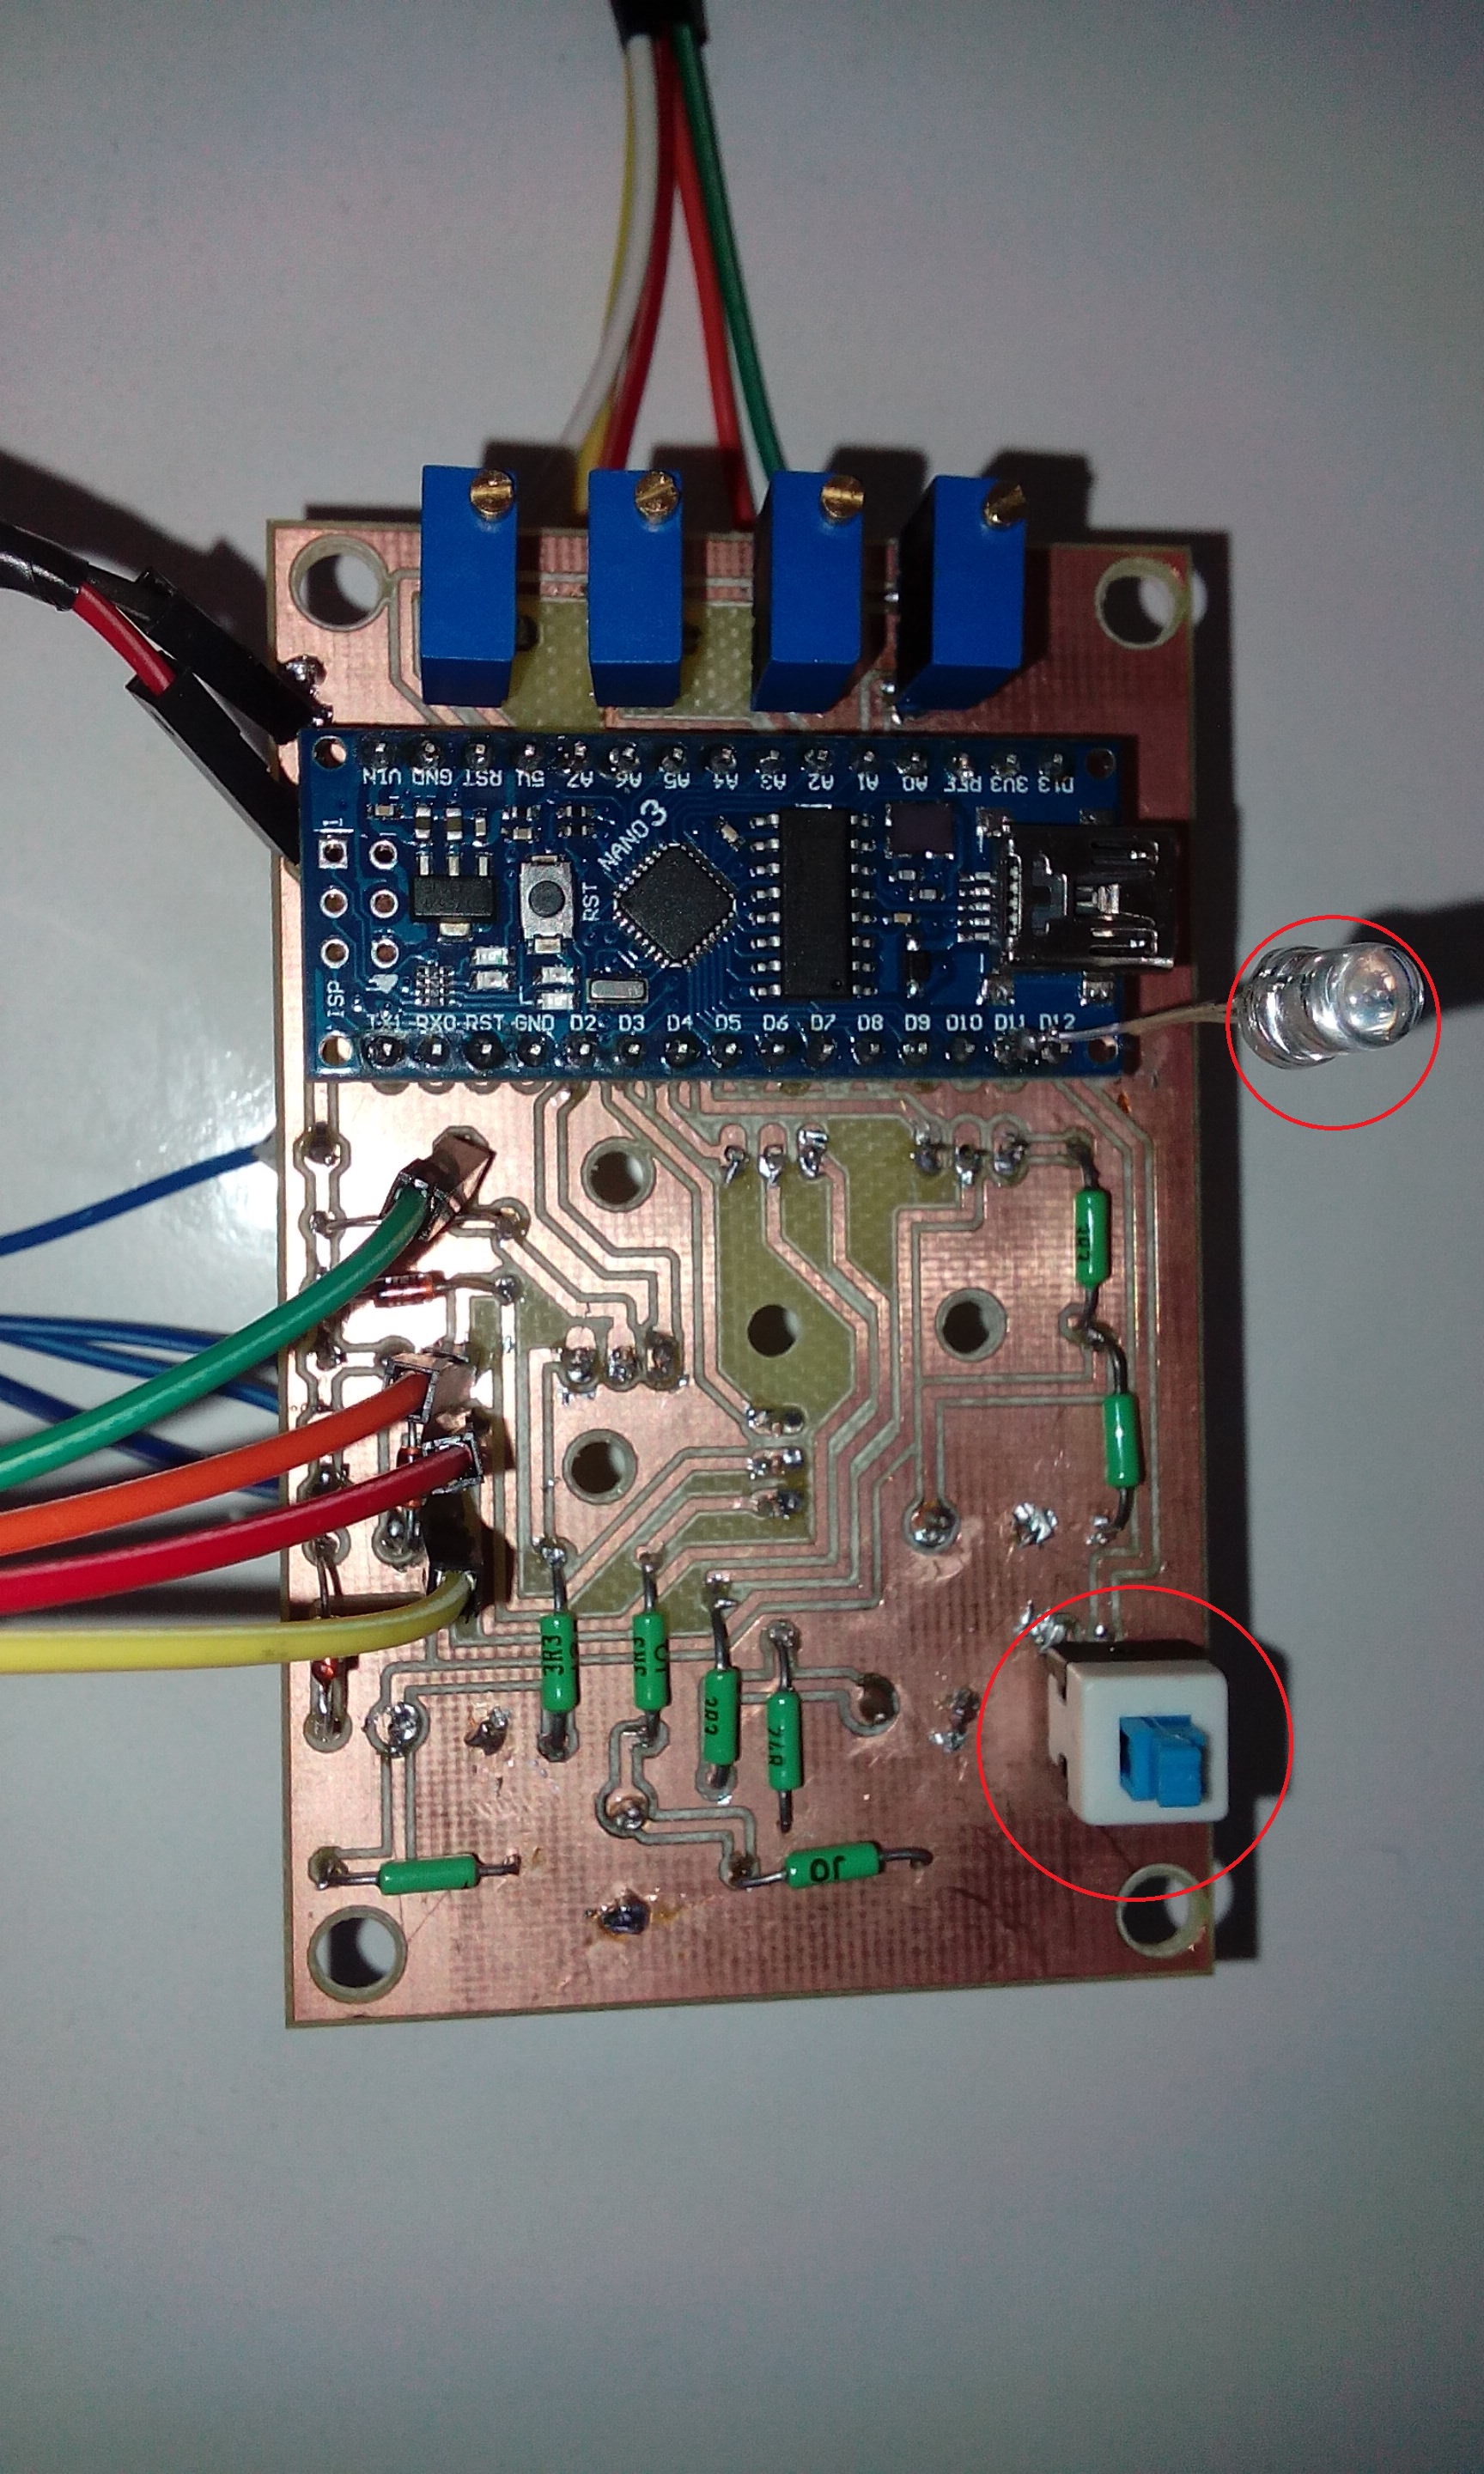
\includegraphics[width=1.00\textwidth]{./img/Navod.jpg}\\[1cm] 
\caption{Nahoře signální LED, dole tlačítko ke kalibraci a ovládání}
\label{Navod}
\end{figure}  

\chapter{Problémy}\label{progProb}
\section{Problémy na které jsme narazili}
\qquad Největším problémem, který stále ještě není dokonale odladěný, byl stisk dlouhých dlaždiček. Designeři hry nám ovšem nabídli ruku v tom, že tyto dlaždice mají jako jediné postupný přechod z černé na modrou (narozdíl od obyčejných dlaždic, které mají přechod skokový). \par \qquad Toho jsme využili a vytvořili se tři úrovně signálu. Rychlost přechodu mezi těmito úrovněmi potom určuje typ dlaždice. Důvod proč tento problém zatím není úplně vyřešený je ten, že některé takové dlaždice jsou příliš krátké a tak se snímaný signál nezdrží v určovací oblasti dost dlouho. Držení těchto dlaždic ale není nutné, takže jsme tomuto problému nedávali příliš velkou prioritu. \par
\qquad Dalším problémem byli nekonsistentní snímače, ačkoliv všechny LDR byli stejného typu, všechny měli jinou závislost odporu na světle. To jsme vyřešili použitím potenciometrů místo rezorstrů v našem zapojení odporových děličů. \par
\qquad Z čehož vyplývá další problém a to absolutní kalibrace PianoTilesMastera. Pokud se s ním nějak hrubě hýbalo nebo se dlouho nepoužíval, je potřeba připojit PianoTilesMaster do počítače a vyrovna úrovně všech senzorů k referenčnímu senzoru (první z prava), to jde udělat velmi lehce přes Arduino IDE plotter.

\chapter{Výsledek}\label{progVys}
\section{Plody našeho projektu}
\qquad V momentě kdy tuhle blbost píšu se PianoTilesMaster dokáže dostat na 10,5 cm/s (nebo v jakých jednotkách ta hra běží) a vlastně chybuje proto, že je přiliš rychlý. Musíme pamatovat, že největším bottleneckem v celém projektu je rychlost FPS mobilu na kterém PianoTiles2 hrajeme. Už od 8 cm/s jsou dlaždičky rozmazané. \par 
\qquad Otázkou je, jak moc se dá PianoTilesMaster doladit a o kolik rychleji ještě bude schopný hrát, to se ale uvidí až se do pořádného ladění pustím, ale prozatimní rychlost je i tak celkem slušná.
\section{Do budoucna...}
\qquad Pokud se k PianoTilesMasterovy ještě v budoucnu vrátím určitě bych vylepšil detekci dlouhých dlaždic, upravil bych kalibraci tak aby byla blbuvzdorná a ještě víc ho doladil aby zvládal hrát co nejdéle. To je ale zatím ve hvězdách.
\part{Shrnutí a závěr}\label{shrnuti}

%%%%%%%%%%%%%%%%%%%%%%%%%%%%%%%%%%%%%%%%%%%%%%%%%%%%%%%%%%%%%%%%%%%%%%%%%%%%%%%%%
%%%%%%%%%%%%%%%%%%%%%%%%%%%%%%%%%%%%%%%%%%%%%%%%%%%%%%%%%%%%%%%%%%%%%%%%%%%%%%%%%
%%%%%%%%%%%%%%%%%%%%%%%%%%%%%%%%%%%%%%%%%%%%%%%%%%%%%%%%%%%%%%%%%%%%%%%%%%%%%%%%%
%%%%%%%%%%%%%%%%%%%%%%%%%%%%%%%%%%%%%%%%%%%%%%%%%%%%%%%%%%%%%%%%%%%%%%%%%%%%%%%%%
\part{Přílohy a zdroje}\label{Pril_zdr}

\chapter{Přílohy}\label{Prilohy}

(1) Mechanická část - Návrh modelu v prostředí Autocad a nákresy jednotlivých částí v pdf\\
(2) Plošný spoj - včetně schématu vytvořený v prostředí Eagle\\
(3) Řídící obvod - Návrh v prostředí Matlab Simulink a spouštěcí m-file\\
(4) Datasheety - Přiložené datasheety pro elektronické komponenty\\


\begin{thebibliography}{9}

\bibitem{grabcad} 
GRABCAD COMMUNITY,
\textit{3D model použitého solenoiu}
\\\texttt{https://grabcad.com/library/tag/rob-11015}

\bibitem{latex} 
Overleaf,
\textit{Návody k prostředí \LaTeX\ }
\\\texttt{https://www.overleaf.com/learn}

\bibitem{mathworks} 
MathWorks,
\textit{Návody k prostředí Matlab }
\\\texttt{https://www.mathworks.com/}

\end{thebibliography}
\end{document}
